\chapter{Test and Performance}\label{ch:testAndPerformance}
\section{Setup}\label{sc:setup}
To test our original scenario described in the Introduction on page \pageref{ch:introduction} we built a smaller version of the running track. To get a constant speed and a track to run tests on we use a Brio\texttrademark train to symbolism a human runner that runs a track. The speed of the runner was set to $12\dfrac{km}{hr}$ but the Brio train had a speed of $0.2604\dfrac{km}{hr}$. The track we used in the theory part was 906.17m long and the runner would run a marathon which is 46.56km and therefor is 46.56 rounds. Using the standard Brio track pack we build a track with length of 43.5cm. In the theory we send $4\dfrac{packets}{sec}$ and that means our time per packet should be $\dfrac{1}{4sec} = 0.250ms$ and therefor about $ 1.087*10^3$ packets per round. But our as our train is slowing than the runner and the track was shorter we needed to account for the differences between our test setup and the theory made in section \ref{table:datascenarios} on page \pageref{table:scenarios}. Our inital calulations showed that we needed to send XXX packets and that was not possible use to limits of the hardware, as seen in Figure POWERFIFG REF it takes 15ms to send a packet and that is not accounting for other things the TelosB might be during so as handling computations. Therefor we divided the packets per round by 4 $ \dfrac{packetsPerRound}{4} = 271.852 $ and therefor needing $57.016 ms$ per packet



\begin{figure}[H]
	\centering
	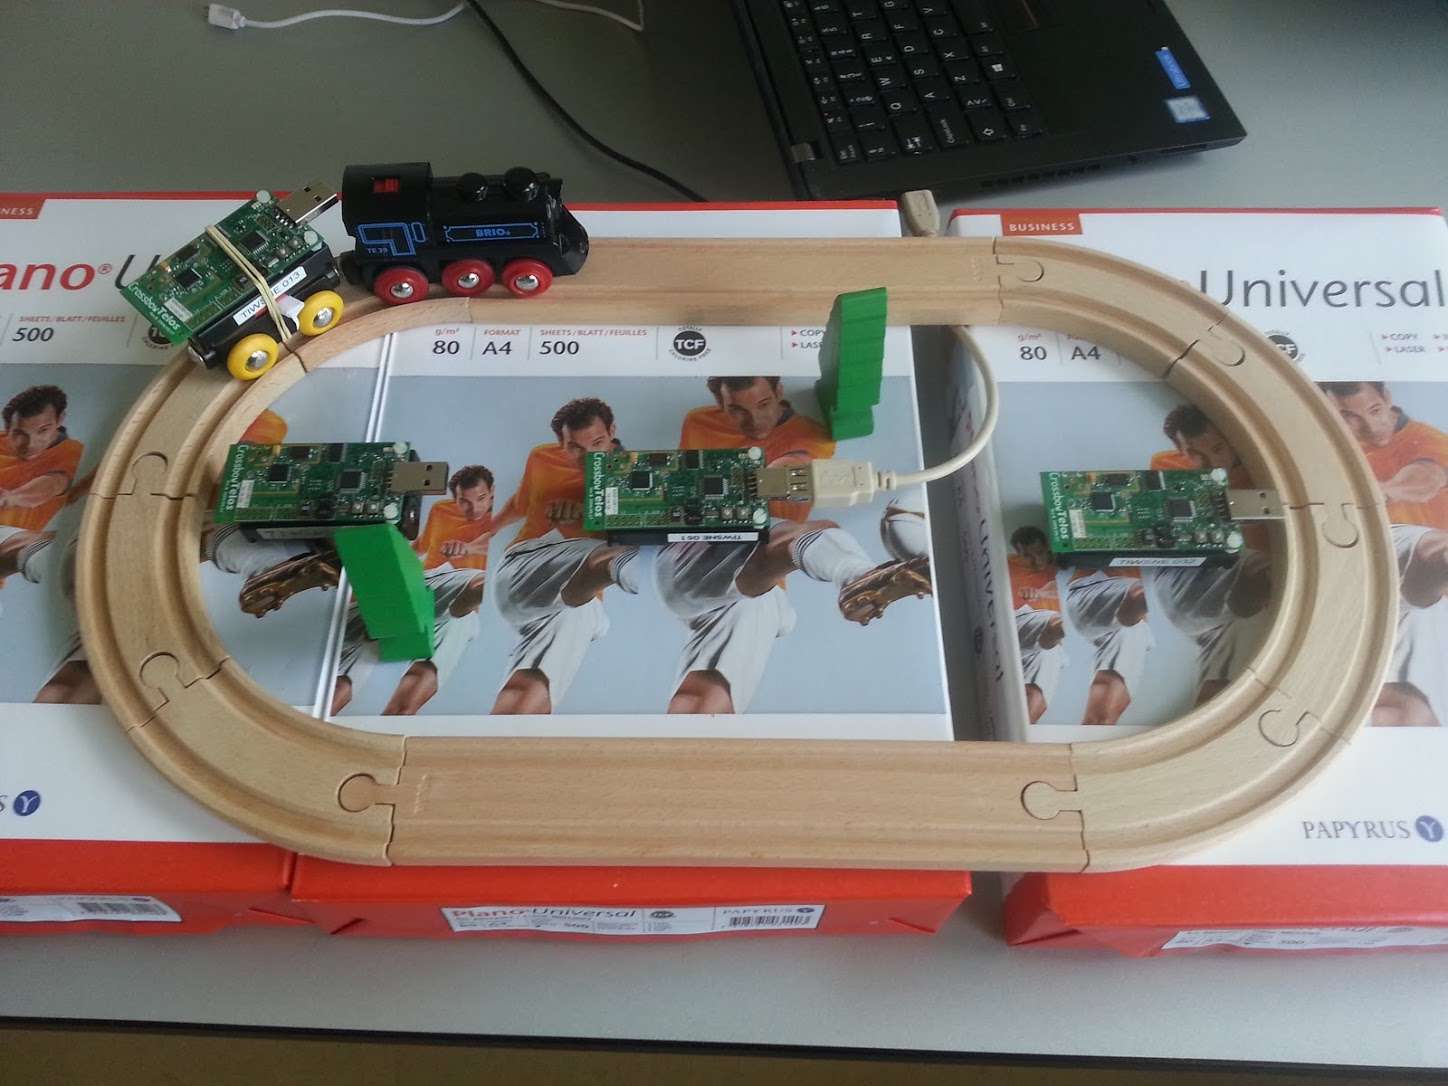
\includegraphics[width=1\linewidth]{testAndPerformance/setup/setup}
	\caption{The train track withbasestation, north and south relay nodes and the runner. }
	\label{fig:testSetup}
\end{figure}


\begin{figure}[H]
	\centering
	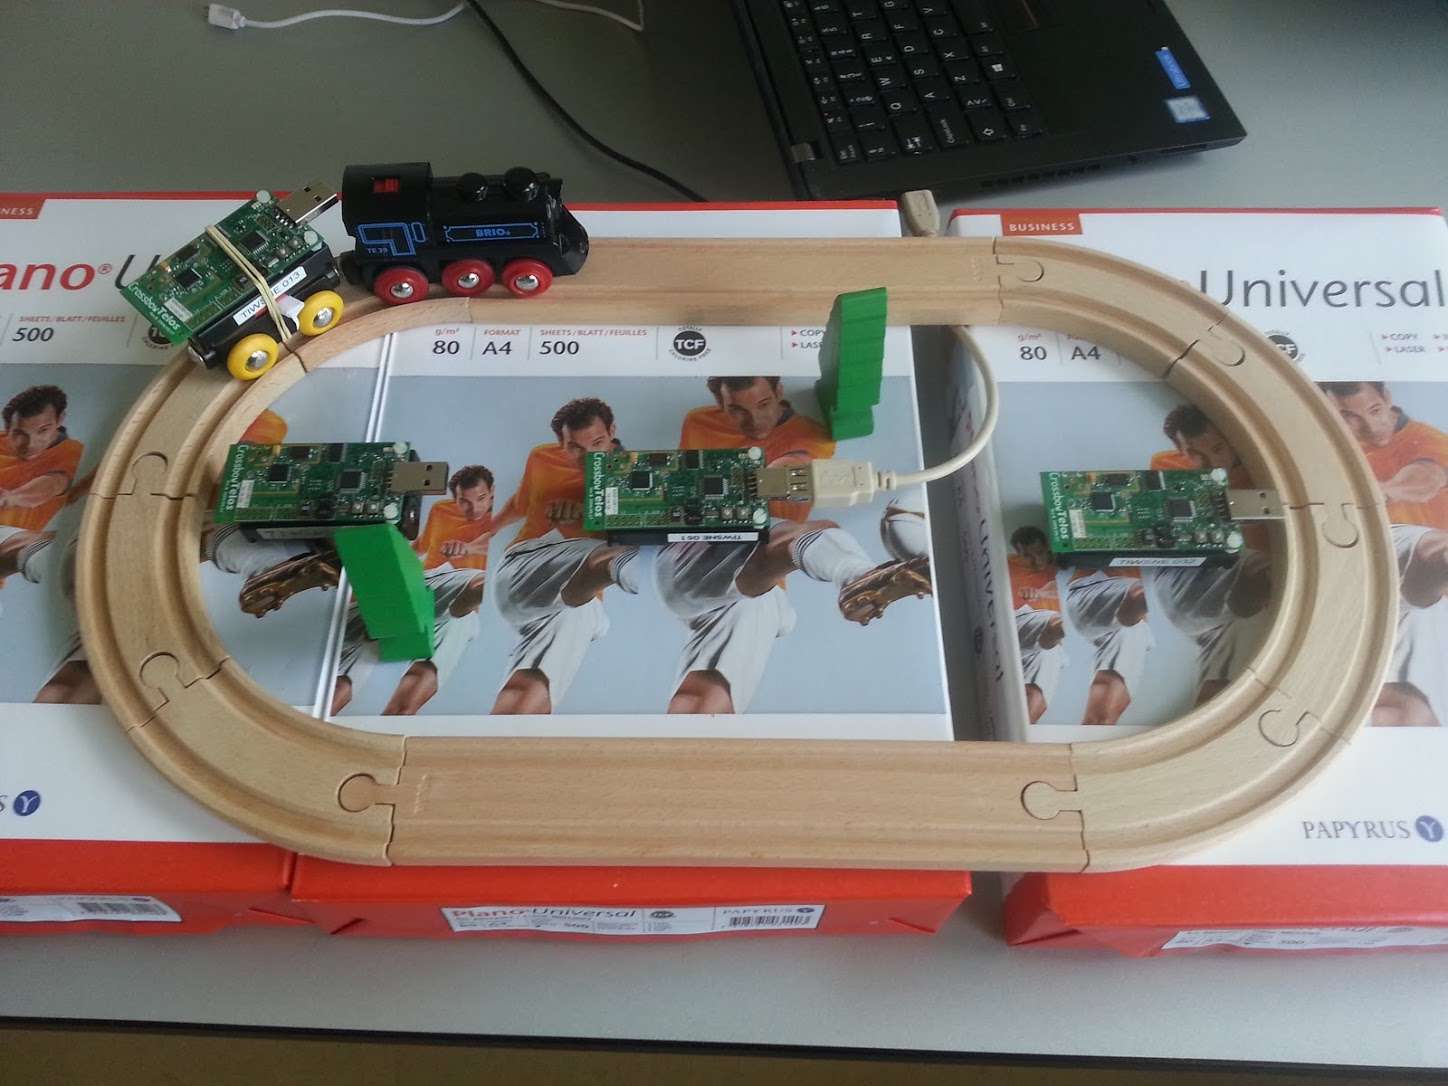
\includegraphics[width=1\linewidth]{testAndPerformance/setup/setup}
	\caption{The train track withbasestation, north and south relay nodes and the runner. }
	\label{fig:testSetup}
\end{figure}


\section{WiFi conditions}\label{sc:wifi}
In our test we used two different WiFi chanenls (4 and 11) and we found the best and the worst by using the WiFi Analyzer app from the Android app store\cite{Farproc@gmail.com2018}. As seen in figure \ref{fig:wifionthetestday}, channel 11 is used by Aarhus University WiFi but channel 4 looks rather free, so we picked these two as seen in table \ref{table:scenarios}.

\begin{figure}[h]
	\centering
	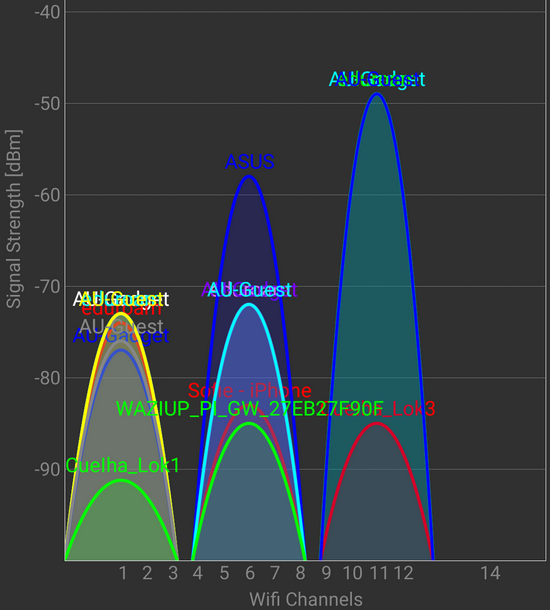
\includegraphics[width=0.6\linewidth]{testAndPerformance/wifi/wifiOnTheTestDay}
	\caption{WiFI on the test day. Channel 11 was busy and Channel 4 was a quiet channel}
	\label{fig:wifionthetestday}
\end{figure}

We ran 4 tests for 48 minutes each testing our protocol with different channels and track lengths.

\begin{table}[H]
	\centering
	\begin{tabular}{|l|l|l|l|l|l|l|} \hline
		Scenario & \pbox{18cm}{Channel} & \pbox{18cm}{RSSI} & \pbox{18cm}{Length of track} \\ \hline
		1 & 11 & -40 & 43.5cm \\ \hline
		2 & 11 & -40 & 56cm \\ \hline
		3 & 4 & -40 & 43.5cm \\ \hline
		4 & 4 & -40 & 56cm \\ \hline
	\end{tabular}
	\label{table:scenarios}
	\caption{Four test scenarios using channel 11/4 and different track lengths.}
\end{table}